% !Mode:: "TeX:UTF-8"
% !TEX program  = xelatex
\documentclass[AutoFakeBold,AutoFakeSlant,scheme=plain,degree=bachelor,zihao=-4]{sustechthesis}
% !Mode:: "TeX:UTF-8"
% !TEX program  = xelatex

% 数学符号与环境
\usepackage{amsmath,amssymb}
  \newcommand{\dd}{\mathrm{d}}
  \newcommand{\RR}{\mathbb{R}}
% 参考文献
\usepackage[style=gb7714-2015]{biblatex}
  \addbibresource{ref.bib}
% 无意义文本
\usepackage{zhlipsum,lipsum}
% 列表环境设置
\usepackage{enumitem}
% 浮动题不越过 \section
\usepackage[section]{placeins}
% 超链接
\usepackage{hyperref}
% 图片,子图,浮动题设置
\usepackage{graphicx,subcaption,float}
% 抄录环境设置,更多有趣例子请命令行输入 `texdoc tcolorbox`
\usepackage{tcolorbox}
  \tcbuselibrary{xparse}
  \DeclareTotalTCBox{\verbbox}{ O{green} v !O{} }%
    {fontupper=\ttfamily,nobeforeafter,tcbox raise base,%
    arc=0pt,outer arc=0pt,top=0pt,bottom=0pt,left=0mm,%
    right=0mm,leftrule=0pt,rightrule=0pt,toprule=0.3mm,%
    bottomrule=0.3mm,boxsep=0.5mm,bottomrule=0.3mm,boxsep=0.5mm,%
    colback=#1!10!white,colframe=#1!50!black,#3}{#2}%
\tcbuselibrary{listings,breakable}
  \newtcbinputlisting{\Python}[2]{
    listing options={language=Python,numbers=left,numberstyle=\tiny,
      breaklines,commentstyle=\color{white!50!black}\textit},
    title=\texttt{#1},listing only,breakable,
    left=6mm,right=6mm,top=2mm,bottom=2mm,listing file={#2}}

% LaTeX logo
\usepackage{hologo}
% code highlight
% \usepackage{minted}
\usepackage{abbrevs}
\makeatletter
\renewcommand\maybe@space@{%
  \maybe@ictrue % <= this is new
  \expandafter   \@tfor
    \expandafter \reserved@a
    \expandafter :%
    \expandafter =%
                 \nospacelist
                 \do \t@st@ic
  \ifmaybe@ic % <= this is new
    \space
  \fi
} % 导言区
% !Mode:: "TeX:UTF-8"
% !TEX program  = xelatex
\设置信息{
%   键 = {{中文值}, {英文值}},
    分类号 = {{}, {}},
    编号 = {{}, {}},
    UDC = {{}, {}},
    密级 = {{}, {}},
    题目 = {{}, {\scalebox{0.84}{Real-time Capturing of System Calls on ARM}}},
    子标题 = {{}, {}},
    姓名 = {{}, {Haonan Li}},
    学号 = {{}, {11712510}},
    系别 = {{}, {Computer Science and Engineering}},
    专业 = {{}, {Computer Science and Technology}},
    指导老师 = {{}, {Fengwei Zhang, Associate Professor}},
    时间 = {{}, {2021.6.3}},
}
 % 论文信息
\newabbrev\TheName{\textsc{Syscord}}
\newabbrev\CoreHook{\textit{core hook}}
\newabbrev\Filter{\textit{filter}}
\newabbrev\RecordBuffer{\textit{record buffer}}
\newabbrev\syscall{syscall}
\newabbrev\SysCall{Syscall}
\newabbrev\Syscall{Syscall}


\linespread{1.25}
\begin{document}

% \英文标题页
% \英文诚信承诺书
\摘要标题
% !Mode:: "TeX:UTF-8" !TEX program  = xelatex

\begin{英文摘要}{Linux, Syscall, Record}
    Bug diagnosis is difficult. The first step of bug diagnosis is to reproduce the bug. In areas such as application development, developers usually can only rely on the report logs uploaded by the user to try to reproduce bugs.
    Unfortunately, it is still challenging to reproduce bugs that occurred in the production environment at the development environment. The primary obstacle of reproduction is non-deterministic events at runtime, such as system calls. Hence,  the same execution may lead to different results.

    In this thesis, I present \TheName, a practical tool for recording system calls on Linux. \TheName utilizes Linux tracepoints to hook system calls.
    \TheName collects relevant information for each system call related to their effects, which further helps developers reproduce and fix bugs. I implement a prototype of \TheName and evaluate it with real-world applications. The result demonstrates \TheName capturing system calls completely and efficiently. 
\end{英文摘要}
 % 论文摘要

\目录\clearpage % 目录及换页

\section{Intoduction}
The program often fails. To sufficiently understand and prevent failures,
developers requires firstly reproduce these bugs, which ensures the same output
and bugs. However, directly
re-exection is not suitable for non-deterministic failures, as they may not
appear in a re-execution procedure. Non-deterministic failures are the
consequence of non-deterministic instructions. 

Instructions for running a program can be divided into two categories. One is
deterministic, which means the behavior of deterministic instruction is determined in each
execution. The other type is non-deterministic, meaning that execution in
different situations will have different results. Although most of the CPU
execution is deterministic (e.g., \texttt{ADD}), non-deterministic instructions (e.g., get user input) are also pervasive.
Typical sources of nondeterminism include system calls, interrupts, signals, and
data races for concurrency programs \cite{ronsse_recplay_1999}. All these non-deterministic events can be futher classified into two types:
inconstancy of the data flow - for example, certain system calls such as
\texttt{getrandom} and \texttt{getpid}, and inconstancy of the control flow
- for example, concurrency bug due to memory access in inconsistent order \cite{getrandom2}.

Record-and-replay is a type of approaches that addresses this challenge. Most
Record-and-replay systems work by first recording non-deterministic events
during the original run of a program and then substituting these records during
subsequent re-execution. Record-and-replay system could ultimately guarante that
each replay will be identical with the initial version. The fact that a number
of replay systems have been built and put into use in recent years illustrates
the value of record-and-replay systems in practice \cite{203227,replay_survey,altekar_odr_2009,bhansali_framework_2006}.

% There are several ways to capture calls online at runtime: \textbf{PinPlay}, \textbf{REPT}, \textbf{rr}

There is a rich amount of research on record-and-replay systems, and we can find
their various treatments of non-deterministic records. Early record-and-replay
systems tend to use virtualization techniques so as to observe and record the
entire program non-deterministically on the hypervisior, but the virtual machine
is very heavy \cite{dunlap_revirt_2003, dunlap_smp-revirt_2008}. Some systems
use dynamic binary instrumentation to get the results after running each
instruction, but this is very inefficient \cite{bhansali_framework_2006}. There
are some other systems that choose not to record at runtime in order to address
the expensive cost of recording; instead, they infer these non-deterministic
events based on the control flow and other information collected
\cite{altekar_odr_2009,cui_rept_2018}. However, inference often does not
reproduce program execution as faithfully as records, and the time required for
inference, which in the worst case is a search of the entire space, is a problem
\cite{replay_survey}. There are also systems that use custom hardware, which
inevitably affects its usefulness in practice \cite{montesinos_capo_2009}.
Recently there have been some practical systems that have adopted tools provided
by Linux for tracing, thus achieving better efficiency. Nevertheless, it still
introduces a considerable overhead (50\%) and is therefore used in scenarios
where the developer exactly needs to debug \cite{203227}.

This thesis focuses on the data record part of record-and-replay systems, precisely, the recording of non-deterministic events caused by system calls. I argue that a \textit{practical} record system should  (1) run online, meaning that the recording has little performance impact on the execution of the target program, (2) log all data without any omission, (3) work on commercial off-the-shelf hardware, (4) not require any modification to the target program, and also (5) not require any modification to the kernel.

In this thesis, I propose \TheName, a practical solution for syscall capturing. 
It works with unmodified Linux programs on commercial off-the-shelf (OTS) hardware. My original design was on the ARM platform, but the system can be applied to other platforms as well (e.g. x86, riscv). I demonstrat its usefulness on both x86 and ARM platforms. \TheName consists of three component: \CoreHook, \Filter and \RecordBuffer.

The \CoreHook is a probe of system call. \CoreHook inspects each system call,   and collects the effects on memory and registers by considering the semantics of system calls. The \Filter stores relevant information of the process what issues the system call, and compares this information with the characteristics specified by the developer. The \RecordBuffer temporarily store the recording of system calls and dumps it to file.

We implement a prototype of \TheName{} and evaluate it with the 
aforementioned requirements in mind. The evaluation results show that
\TheName{} completely records system calls. 
% We also leverage \TheName{} to diagnose 16 failed programs (7 code segments 
% reconstructed from application and 9 real-world applications including Python, Memcached, 
% and SQLite). The diagnosis indicates that \TheName{} effectively identifies the root cause 
% of the failures caused by concurrency and sequential bugs
We also leverage \TheName to record 16 failed programs (7 code segments 
reconstructed from application and 9 real-world applications including Python, Memcached, and SQLite). The recording indicates that \TheName effectively records system calls
 with a performance overhead of
up to 3.88\% on average. Meanwhile, \TheName{} directly works on the unmodified binary of the target 
program and does not rely on any hardware modification.

% The main challenge confornt to \TheName is how to 

% I implement \TheName in three components. The hook component is a couple of callback functions that hooks the entrance and exit of each system call. The filter component are  functions 

In summary, I make the following contributions:
\begin{itemize}
    \item I present a system call recording tool named \TheName{} on Arm platforms. To the
    best of our knowledge, it is the first hardware-assisted system call recording tool
    for Arm architecture. 
    \TheName{} works with
    unmodified binary on Arm platform without hardware modification.
    %, thus
    %suitable for in-production deployment.
    \item I achieve high performance that allows the
    always-on trace for the production environment, which provides \TheName{} the ability
    to reconstruct the entire records.
    %so \TheName accurately
    %reconstructs control flow based on the trace and the program binary.
    % \item \TheName{} performs \Adaptivedata{} at \Analysisstage{}, and
    % helps developers to reproduce and locate the \bof{}s that occurred in 
    % the production environment.
    %I propose \Adaptivedata to recover complete data flow in
    %\Analysisstage.
    %To achieve this goal, I utilize the records of \Recordingstage
    %to identical re-execute and reproduce bugs. 
    % \TheName adaptively adds
    % hardware watchpoint/breakpoint to produce coredumps to recover data flow.   
    \item I implement a prototype of \TheName{} and evaluate it with
    buggy real-world applications.
    The evaluation result demonstrates that \TheName{} successfully records
    various types of applications with up to 3.88\% runtime
    performance overhead on average.
  \end{itemize}
  
\section{Background}

\subsection{Linux Tracepoint}



 Tracepoint is a lightweight hook for events provided by Linux. With tracepoint, we can provide a callback function (called a probe) at runtime for Linux to execute when these events are triggered. \cite{torvalds_torvaldslinux_2021,using_tracepoint}

There are two events (\texttt{sys\_enter} and \texttt{sys\_exit}) defined in \texttt{/include/trace/} \texttt{events/syscalls.h} that can be exploited to execute callback function in the procedure of invloking syscall. \cite{torvalds_torvaldslinux_2021}

\subsection{Linux Process Management}

Linux uses process descriptors to represent all information about each process, such as the process priority, the address space allocated, the files allowed to be accessed, and so on. Process descriptors are all of type \texttt{task\_strcut}.  \cite{torvalds_torvaldslinux_2021,bovet_cesati_2006}

In Linux kernel, there is a macro named \texttt{current} defined in \texttt{arch/arm64/include/} \texttt{asm/current.h} (on Arm64). \texttt{current} is a pointer that refers to the process that is currently executing; precisely, the issuer of the system call. \cite{corbet_linux_2005,torvalds_torvaldslinux_2021}
% \section{Overview}

The overarching target of \TheName is to capture Linux syscalls with low overhead. \TheName realizes syscall capturing in three steps. (1) \TheName inspect and record each syscall. (2) Next, \TheName filter these records by some arrtibutions of its caller process. (3) Finally, \TheName transfer these filtered records.

\subsection{Design Choices}

When designing \TheName, I make three design choices.

\begin{itemize}
    \item \textbf{Modify Kernel Source vs. Load Kernel Module:} Modifying Kernel source may make all procedures much more easy. However, this approach will inevitably reduce the compatibility of \TheName, especially for devices whose kernels have been modified by manufacturers. Futhermore, to modify kernel, we would also need to synchronize upstream changes. Consequently, \TheName is baesd on kernel moudle and works as a loadbale driver.
    \item \textbf{Source vs. Binary: }  I choose to do the capturing at
    the binary level instead of at the source code level. because it is quite common that source code and system calls have not corresponded (e.g., library function \texttt{malloc} do not necessarily call the \texttt{mmap}), with most programs use libraries instead of calling system calls directly. In fact, \TheName only concerns the runtime of processes, and would not perform any static analysis.
\end{itemize}

\subsection{Challenges}

To achieve its desgin goal, \TheName faces following challenges.


\subsubsection{Syscall parameters}

Considering some syscalls that allow to pass pointer and then modify its memory addressed by this pointer, it is necessary to check and record the change. For example, the prototype of syscall \texttt{getrandom} is defined as follow:\cite{getrandom2}


\centerline{\texttt{ssize\_t getrandom(void *buf, size\_t buflen, unsigned int flags);}}

It is clear that the \texttt{getrandom} will fill the buffer pointed to by its first parameter, \texttt{buf}. Therefore, \TheName needs to record the memory area changed by syscall. However, there is still a challenge that sometimes we cannot get the address at the end of syscall involked. This is due to the way the parameters are passed, determined by the architecture of CPU.

In Arm64 \cite{syscall}, both first argument(\texttt{arg1}) and return value are saved in register \texttt{r0}, which means the parameter stored in \texttt{r0} will be replaced with return value before the syscall return to user. This results in the inability to directly record the chanegs only at the end of syscall handled in kernel. I solve this challenge by adding an extra record for several syscalls.


% \subsubsection{Filter by Process}

% The capture needs filter by process due to the concurrency of the OS, i.e., interleaving with multiple processes. Thus, to distinguish the different syscall callers, \TheName has to add the caller's information for each syscall record. Accordingly, this challenge become \textit{how to get the process that issued the system call}. I address this challenge by inspecting a sepcial data structure in Linux kernel.

\subsubsection{Record Transfer}

System call records need to be stored in a buffer, while it is a very important issue when it comes to somehow get them from the buffer in real-time, with low consumption, and completely. However, the most strightforward solution, i.e., trying to keep fetching data from the buffer and save to file, causes a huge amount of overhead. I solve this challenge by enlarging buffer and reducing the frequency of acquisition.




\section{Design}
The overarching target of \TheName is to capture all syscalls issued by target application with low overhead. Specifically, it has the following characteristics:

\begin{itemize}
    \item \textbf{online:} Our scenario is that our entire record system can  run simultaneously on the user side and eventually become a part of the log report. Therefore it must introduce only a extremely low overhead to guarantee that the user can run the desired program without perception.
    \item \textbf{complete:} We also need to ensure the integrity of record results, i.e. that every syscall is correctly captured with all the data needed for reproduction. Not only do we need to verify the correctness of our records on each syscall, but we also have to guarantee that the data in the buffer is fetched in a timely manner without any overflow.
    \item \textbf{off-the-shore:} An practical system should never make assumptions about the hardware. \TheName is desgined completely based on the off-the-shelf hardware.
    \item \textbf{without modification to application:} We do not make any changes to the source code or binary of the target application. The entire code of our system runs in kernel space, except for the transfer of logged results that need to be transferred to user space. This means that \TheName cares nothing about how the target application in user space is executed, but only about the event that this target application jumps to the kernel state.
    \item \textbf{without modification to kernel:} Modifying Kernel source may make all procedures much more easy. However, this approach will inevitably reduce the compatibility of \TheName, especially for devices whose kernels have been modified by manufacturers. Futhermore, to modify kernel, we would also need to synchronize upstream changes. Consequently, \TheName is baesd on kernel moudle and works as a loadbale driver.
\end{itemize}


\TheName realizes syscall capturing in three steps. (1) \TheName inspect and record each syscall. (2) Next, \TheName filter these records by some arrtibutions of its caller process. (3) Finally, \TheName transfer these filtered records.

\begin{figure}
    \centering
    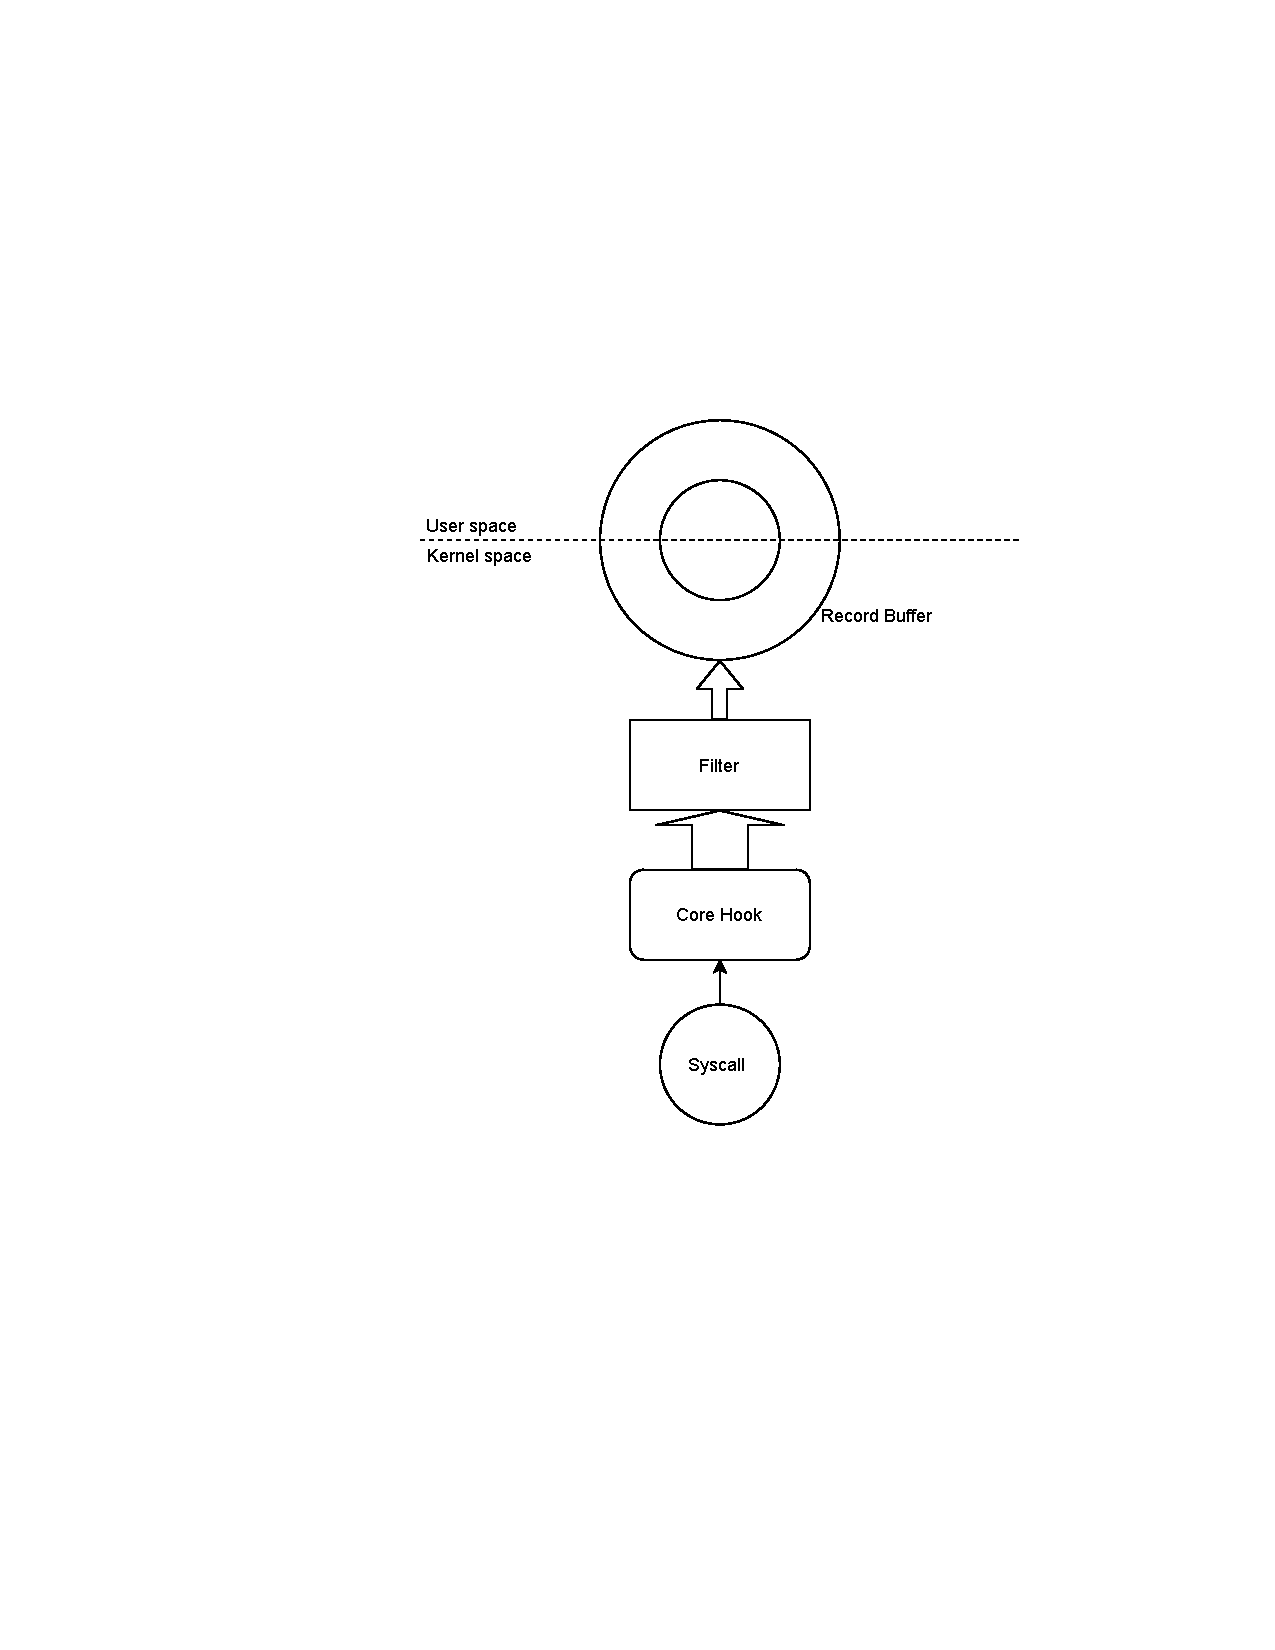
\includegraphics[width=0.8\textwidth]{figures/arch.pdf}
    \caption{The Overview of \TheName}
    \label{fig:arch}
\end{figure}



% In this section, I describe the desgin of \TheName by focusing on how it solves the above challenges

\subsection{Desgin Overview}

In this section, I present the desgin of \TheName by focusing on how it addresses the above two key challenges. \TheName contians three parts: \textit{core hook}, \textit{filter}, and \textit{record buffer}. 

As Figure \ref{fig:arch} shows, in the kernel space, \textit{core hook} collect information for each system call, and then transfer to \textit{filter} part. Subsequently, at the \textit{filter} part, it will find process information from the kernel, and filter syscall records with specific features (e.g., process id or name) and finally pass to \textit{record buffer}. The record buffer manage the buffer in kernel space and file write to user space.


\subsection{Case Study}

\begin{figure}
    \begin{minipage}[t]{0.46\textwidth}
      \begin{lstlisting}
  // Thread 1::
  char big_buf[64];
  while(1)
    read(fd, big_buf, 64);
      \end{lstlisting}    
    \end{minipage}
    \begin{minipage}[t]{0.46\textwidth}
      \lstset{firstnumber=last}
      \begin{lstlisting}
  // Thread 2::
  int total = 0;
  int len = 0;
  char buf[15];
  for (short i=0; i < 2; ++i)
    len = strlen(big_buf);
    if (len < 15)
      strcpy(buf, big_buf);
      total += len;
  assert(total<30)
    \end{lstlisting}    
    \end{minipage}
  
  
    \caption{Buffer Overflow Caused by Data Race}
    \label{fig:data-race}
\end{figure}

Figure~\ref{fig:data-race} demonstrates a typical concurrency
bug related to the 
\syscall{} \texttt{read}. Assume that the loop (Line 10 to Line 13) in Thread 2
is executed twice. In the first iteration, the \texttt{read} of 
\texttt{big\_buf} (Line 4) in Thread 1 is performed after the length 
check (Line 10 and Line 11) in Thread 2. The following \texttt{strcpy} (Line 12) in 
Thread 2 may lead to a buffer overflow and overwrite variables \texttt{len} and 
\texttt{total}. In the second iteration, no data race is involved, but the 
unpredictable \texttt{total} overwritten in the first iteration might be larger
than 30 after the summation (Line 13) in Thread 2. This finally fails the
\texttt{assert} (Line 14) in Thread 2 and crashes the program.
In this example, the memory and registers indicating the root cause of
the bug are overridden by subsequent control flow. 
Hence, it is necessary to record the content of syscall \texttt{read} to figure out the bug.


\begin{figure}
    \centering
    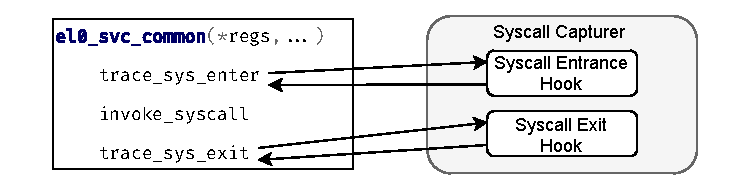
\includegraphics[width=0.95\textwidth]{figures/syscall_capturer.pdf}
    \caption{The Two hooks of \textit{core hook}}
    \label{fig:core-hook-desgin}
\end{figure}

\begin{table}
    % table caption should be in the top.
    \caption{
        Part of Registers Used in Syscalls \cite{syscall}.}
    \centering
    \begin{tabular}{lllllll}
        \toprule
        arch                      &  syscall number &
        return value &
        return value 2 & arg0                      & arg1 &
        arg2                                                               \\
        \midrule
        ARM64                     & w8                        & x0   & x1
                                  & x0                        & x1   & x2  \\
        x86-64                    & rax                       & rax  &
        rdx                       & rdi                       & rsi  & rdx
        \\
        RISC-V                     & a7                        & a0   & a1
                                  & a0                        & a1   & a2  \\
        \bottomrule
    \end{tabular}
    \label{table:arch_registers}
\end{table}


\subsection{Core Hook}

\textit{Core hook} utilizes \textit{Linux Kernel Tracepoints} \cite{mathieu2021using}, which
provides lightweight hook points in critical positions over the kernel
(includes the enter and exit of \syscall{}), to achieve the capture.  Figure \ref{fig:core-hook-desgin} illustrates the procedure of \syscall{}s
(defined at function \texttt{el0\_svc\_\\common} for ARM64) and the recording for \syscall{}s. 


When entering a \syscall{}, the kernel goes into \textit{syscall entrance
hook} which stores values of involved registers. As Table
\ref{table:arch_registers} shows, the register \texttt{x0} and \texttt{x1} are used as both
parameters and return values of \syscall{}s on ARM64. Thus, these registers are
overwritten by return values during \syscall{} procedure. Consequently, we may not
obtain the \syscall{} parameters at the \textit{syscall exit hook} directly.
However, these parameters are critical in some cases. For example, as Figure
\ref{fig:data-race} demonstrates, the content of \texttt{big\_buf}, addressed by
the first parameter of \texttt{read}, is necessary for failure analysis.
Therefore, we need to record the corresponding parameter at the \textit{syscall
entrance hook}, and further record the content addressed by \texttt{big\_buf} at 
the \textit{syscall exit hook}.

Before exiting a \syscall{}, the kernel falls into \textit{syscall exit
hook}. This hook records different information for
various types of \syscall{}s. Firstly, if the capturer notices that a
\syscall{} only changes specific registers (e.g., \texttt{getpid} only changes
return value), it could selectively save information to reduce the size of
record file. Secondly, we need to record additional information for
certain \syscall{}s;
for example, the \syscall{} \texttt{read(int fd, void *buf, size\_t count)}
tries to fill \texttt{count} bytes to the memory region addressed by
\texttt{buf}. In this case, we have to notice and record the write to this
memory region. 

For a better understanding of the impact of \syscall{}s, we classify
them into four types according to their effect on memory and registers.

\begin{itemize}
\item
\noindent\textbf{R}\textit{eading} \textbf{S}\textit{tatus}: 
The \textit{RS-Type} \syscall{}s
aim to read information related to system status. The results of
these \syscall{}s may be transferred by the return value (e.g., \texttt{getpid}), 
a pointer (e.g., \texttt{getitimer}), or shared memory (e.g.,
\texttt{getrandom}). For all \syscall{}s
in this category, we can directly record the memory or register they changed.

\item
\noindent\textbf{W}\textit{riting} \textbf{S}\textit{tatus}: 
The \textit{WS-Type} \syscall{}s
changes the status of the system. As the \textit{WS-Type} \syscall{}s do not
directly change the memory and registers of the program, we ignore
them unless they fail and return an error code. 
For example, the \syscall{} \texttt{epoll\_create} in \texttt{epoll} API
is ignored, but the influence of \syscall{} \texttt{epoll\_wait} is
recorded since we classify it as an \textit{RS-Type} \syscall{}.

%we do not handle \syscall{}
%\texttt{epoll\_create} in \texttt{epoll} API, while we record the influence
%of \syscall{} \texttt{epoll\_wait} as we classify it as \textit{Get from OS}.

\item
\noindent\textbf{R}\textit{eading} \textbf{C}\textit{ontent}: 
The \textit{RC-Type} \syscall{}s read content from an external input, and the
handling of \textit{RC-Type} \syscall{}s is similar to that of \textit{RS-Type} 
\syscall{}s. However, since the content is usually much larger than
the status read in the \textit{RS-Type} \syscall{}s, we choose to
truncate the content and record only the first 256 bytes due to
performance requirements. Recording the entire content may become
impractical in extreme cases (e.g., data center with tremendous
uploads) as it results in a huge size of record file. 
Besides, we find that the truncated content is sufficient for bug diagnosis in
most cases. A further evaluation is discussed in
\S \ref{space-consumption}.

\item
\noindent\textbf{W}\textit{riting} \textbf{C}\textit{ontent}:
The \textit{WC-Type} \syscall{}s write content to an external source. We 
consider that they would not affect the execution status of the target
program. For example, the \syscall{} \texttt{write} is ignored, and
the written content is recorded if the \textit{RC-Type} \syscall{}
\texttt{read} is used to read from the source again.
%The content of \syscall{}s like \texttt{write} or
%\texttt{sendto} also no needs to record, unless it fails.
\end{itemize}



% Table \ref{table:arch_registers}, both first argument(\texttt{arg1}) and return value are saved in register \texttt{r0}, which means the parameter stored in \texttt{r0} will be replaced with return value before the syscall return to user. This results in the inability to directly record the chanegs only at the end of syscall handled in kernel. I solve this problem by adding an extra record for several syscalls.


% \subsubsection{Filter by Process}

% The capture needs filter by process due to the concurrency of the OS, i.e., interleaving with multiple processes. Thus, to distinguish the different syscall callers, \TheName has to add the caller's information for each syscall record. Accordingly, this challenge become \textit{how to get the process that issued the system call}. I address this challenge by inspecting a sepcial data structure in Linux kernel.

% \subsubsection{Record Buffer}

% System call records need to be stored in a buffer, while it is a very important issue when it comes to somehow get them from the buffer in real-time, completely, and with low overhead. However, the most strightforward solution, i.e., trying to keep fetching data from the buffer and save to file, causes a huge amount of overhead. Therefore, I choose to directly write to file 



\subsection{Filter}

The \Filter is responsible for reducing the record size by applying filter conditions, and then only  transfer relevant system calls to \RecordBuffer.
The \Filter can filter the process who issued the syscall by its attributions (e.g., process id, process name, and parent process id), as it leverages \texttt{current} to collect relevant information about the issuer. The \texttt{current} points to the process descriptor \texttt{task\_struct} which contains all the information about the executing process. During a procedure of system call, \texttt{current} pointer indicates the issuer of the syscall \cite{corbet_linux_2005}. 


\begin{figure}
    \centering
    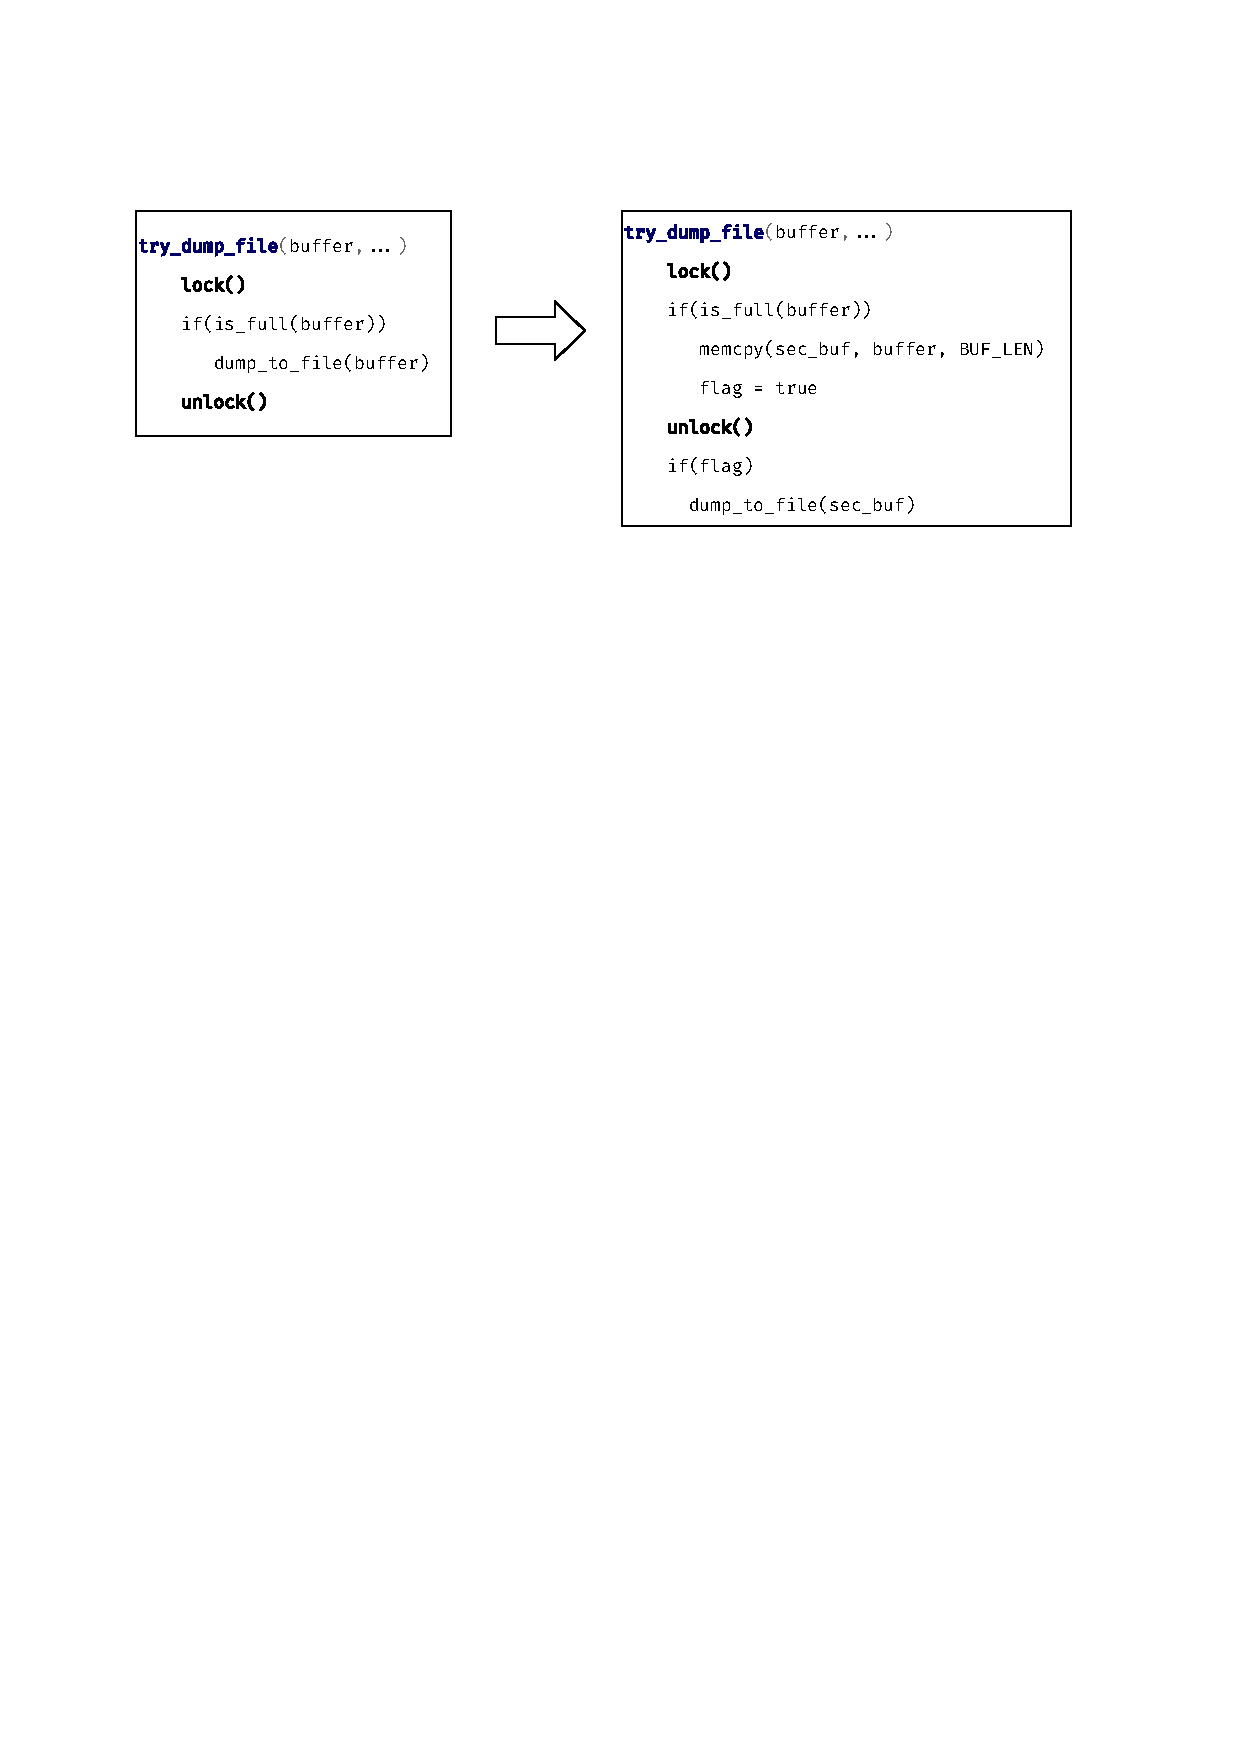
\includegraphics[width=0.9\textwidth]{figures/dual_buf.pdf}
    \caption{The procedure for dumping file}
    \label{fig:dual_buf}
\end{figure}



\subsection{Record Buffer}

The \textit{record buffer} intends to transit between kernel space and user space. As Figure \ref{fig:dual_buf} demonstrates, considering that dumping to a file is relatively slow, the left design of Figure \ref{fig:dual_buf} causes \texttt{dump\_to\_file} to block system calls throughout the entire OS. In contrast, the design on the right only locks the \texttt{memcpy}; after the memory copy, other simultaneous system calls can directly write to \texttt{buffer}. 

There is a risk that the buffer fills up again before \texttt{dump\_to\_file(sec\_buf)}, which makes part of the records lost. However, even in some extreme cases, this risk does not arise. The evaluation results are provided in \S\ref{subsec:eva-flowaccuracy}.


% Therefore, \TheName directly writes to file from the kernel, i.e., when the buffer is full, \TheName dumps the buffer to files. In addition, it is noticeable that the kernel can not write files in all cases. For example, considering system calls that controls files such as \texttt{open}, \texttt{read} or \texttt{close}, \TheName should avoid writing files, or it will induce scheduling while atomic. Hence, \TheName maintains an additional secondary buffer. When the original buffer uses up, its content transfers to the secondary buffer, and then waits for a syscall irrelevant to file management to dumps to file.
\section{Implementation}

In this section, we describe our prototype of \TheName. We implement \TheName
with more than \texttt{1.6k} lines C/C++ code
on an Armv8 board based on Linux. In our prototype of \TheName, we analyze the semantics of the 60 commonly used
\syscall{}s. For each \syscall{}, \TheName generates a description including  return address, process id and its effects. We also use a 16 MB buffer to temporarily store
the \syscall{} records and then dump this buffer to files when it is full. 

To optimize performance, we further apply a simple encoding rule to reduce the size of record file. The \TheName only incurs a low overhead in both time and space. Detailed measurement is presented
in \S ??.

\begin{itemize}
    \item new sprintf
    \item encoding
\end{itemize}

\subsection{Core Hook}


The part of \textit{core hook} aims to hook system call, i.e., inject custom code at the begin and the end of a system call. By leveraging \textit{core hook}, It is easy to get the return value of the system call and the changes to the parameters. Linux has provided many different approaches to achieve it, such as \textit{ptrace}, \textit{auditd}, \textit{Kprobe} and \textit{tracepoint}. 

I choose \textit{tracepoint} to implement our core hook, since it 

% Ptrace is a system call that can be used for many things. By using ptrace,  a process can easily inspect and manipulate the internal state of another program, i.e., the target process. For example, debuggers like gdb can be used to see what processes are running \cite{ptrace2} .

% The ptrace mechanism allows users to interrupt the traced process each time a system call is invoked, and then apply custom analysis. Nevertheless, The challenge is that, each time a system call is invoked, a transition from the user mode to the kernel mode is required. In Linux, it will save and restore a lot of registers (e.g., all general propose registers) at the time entering and exiting kernel mode\cite{torvalds_torvaldslinux_2021}. Therefore, we do not implement \textit{core hook} by ptrace.


% It should be clear why ptrace is not efficient: each original signal mode switch becomes multiple mode switches. Therefore, our \textit{core hook} cannot develop basd on ptrace.

% \subsubsection{auditd}

% It is also very slow.

% \subsection{Kprobe}

% But Kprobe, with too limited in features. Kprobe-based event tracers used by perf, which did not allow the ability to dereference arbitrarily complex structures and severely limited the ability to introduce custom logic in the instrumentation phase


\subsection{Filter}

We get the process descriptor of syscall issuer (the process using the syscall) via \texttt{current}, and compare it with conditions passed in.

\subsection{Record buffer}

The buffer is a circular queue. And there is also a number indicating the usage of the buffer. 

The most sophisticated component is to share the buffer between kernel space to user space. 
\section{Evaluation} \label{sec:evaluation}


In this section, we first use a case study (\S\ref{subsec:eva-casestudy}) given
in Figure \ref{fig:data-race} to show the complete workflow of the \TheName. 
Next, we focus on evaluate \TheName{} with the four practical requirements
discussed in \S\ref{sec:introduction}. Specifically, we aim
to answer the following research questions:

\vspace{1pt}
\noindent\textbf{RQ 1:} How completely can \TheName record system calls? (\S\ref{subsec:eva-flowaccuracy})

\vspace{4pt}
\noindent\textbf{RQ 2:} What is the performance of \TheName? (\S\ref{subsec:eva-Efficiency})

\vspace{4pt}
\noindent\textbf{RQ 3:} Could \TheName perform bug analysis on binary code? (\S\ref{subsec:eva-Generality})


We deploy the \TheName on an Armv8 Juno r2 board equipped with 6 cores (2
Cortex-A72 cores and 4 Cortex-A53 cores) and 8GB RAM based on Linaro
deliverables Linux 5.4.50. We equip the Juno board with an SSD and allocate
256 MB circular buffers for ETM tracing. We use this as the default setting for
our experiment but also allowed developers to adjust it as required.

\subsection{Case Study} \label{subsec:eva-casestudy}


% Please add the following required packages to your document preamble:
% \usepackage{booktabs}
\begin{table*}[]
    \caption{Tailored Control Flow And Data Flow for Figure~\ref{fig:data-race}}
    \label{study_case_flow}
    \centering
    \scalebox{0.62}{
    \begin{tabular}{@{}llll@{}}
        \toprule
        \textbf{Block} & \textbf{Thread 1}                           & \textbf{Thread 2}                                       & \textbf{Data Values}                                          \\ \midrule
        A              &                                             & bl 400910 \textless{}strlen@plt\textgreater{}           & total=0, len=0, buf=?                                          \\
        B              & bl 400960 \textless{}read@plt\textgreater{} &                                                         & read, fd=3, size=64, res=25,  data="1234567890123456789012345" \\
        C              &                                             & bl 400970 \textless{}strcpy@plt\textgreater{}           & total=0, len=875770417, buf=“123456789012345"                  \\
        D              & bl 400960 \textless{}read@plt\textgreater{} &                                                         & read, fd=4, size=64, res=6, data="123456"                      \\
        E              &                                             & bl 400910 \textless{}strlen@plt\textgreater{}           &                                                                \\
        F              &                                             & bl 400970 \textless{}strcpy@plt\textgreater{}           & total=875770423, len=6, buf="123456"                           \\
        G              &                                             & bl 400940 \textless{}\_\_assert\_fail@plt\textgreater{} &                                                                \\ \bottomrule
    \end{tabular}
    }
\end{table*}

To evaluate the functionality of \TheName, we test it with the program shown in
Figure \ref{fig:data-race}. As Table \ref{study_case_flow} illustrates, 
it is clear that Thread 2 checks the length of \texttt{big\_buf} (Line 10, 
Block 2-A) before the first \texttt{read} (Line 4, Block 1-B) in Thread 1. Since 
we capture the data of \texttt{read}, we know that the \texttt{big\_buf} contains 
a string with length 25. Therefore, the following \texttt{strcpy} (Line 12, 
Block 2-C) incurs a buffer overflow, and the variable \texttt{len} (Line 7) 
is unexpectedly changed to \texttt{875770417}, which finally leads to the failure 
of the \texttt{assert} (Line 14, Block 2-G). 

It is notable that the program does not crash immediately after the buffer 
overflow. In contrast, it executes normally for the second cycle (Block D to F). 
In addition, the normal execution of the second time overwrites the 
values (\texttt{buf} and \texttt{len}) involved in the buffer overflow, which 
may confuse developers without the assistance of \TheName.


\subsection{Completeness} \label{subsec:eva-flowaccuracy}



\subsection{Effectiveness} \label{subsec:eva-Effectiveness}

\begin{table}
    \caption{Syscalls issued from bugs recorded by \TheName{}. N/A=bugid is not available, E=reconstructed bug, R=real-world bug, OV=order violaion, SAV=single variable atomicity violation, MAV=multi variables atomicity violation, DL=deadlock, SEQ=sequential bug (non-concurrency bug), LOC=line of code}
    \scalebox{1.0}{
        \begin{tabular}[]{@{}llll@{}}
            \toprule
            \textbf{Program-BugID-GroupType} & \textbf{bug type} & \textbf{LOC} & \textbf{Symptom}         \\
            \midrule
            shared\_counter-N/A-E            & SAV               & 45           & assertion failure        \\
            log\_proc\_sweep-N/A-E           & SAV               & 93           & segmentation fault       \\
            bank\_account-N/A-E              & SAV               & 95           & race condition fault     \\
            jdk1.4\_StringBuffer-N/A-E       & SAV               & 180          & assertion failure        \\
            circular\_list-N/A-E             & MAV               & 155          & race condition fault     \\
            mysql-169-E                      & MAV               & 120          & assertion failure        \\
            mutex\_lock-N/A-E                & DL                & 51           & deadlock                 \\
            SQLite-1672-R                    & DL                & 80K          & deadlock                 \\
            memcached-127-R                  & SAV               & 18K          & race condition fault     \\
            Python-35185-R                   & SAV               & 1256K        & race condition  fault    \\
            Python-31530-R                   & MAV               & 1256K        & segmentation fault       \\
            aget-N/A-R                       & MAV               & 2.5K         & assertion failure        \\
            pbzip2-N/A-R                     & OV                & 2K           & use-after-free           \\
            curl-965-R                       & SEQ               & 160K         & unhandled input pattern  \\
            cppcheck-2782-R                  & SEQ               & 120K         & unhandled input pattern  \\
            cppcheck-3238-R                  & SEQ               & 138K         & NULL pointer dereference \\
            \bottomrule
        \end{tabular}}
    \label{table:bug benchmarks}
\end{table}


We show how effectively \TheName is for diagnosing the root cause of bugs. As
listed in Table \ref{table:bug benchmarks}, we use 16 commonly C/C++ buggy
programs
\cite{cui2018rept,kasikci_lazy_2017,yu2009case,yu2012maple,kasikci2015failure, liang2020ript}
to evaluate \TheName.
% We focus on picking open-source software bugs for
% reproducibility in the Arm platform
We divide these bugs into two groups, i.e., Group E and Group R.
Group E contains 7 bugs reconstructed from
applications \cite{yu2009case,yu2012maple}, and Group R includes 9 bugs in
real-world applications
\cite{cui2018rept,kasikci_lazy_2017, kasikci2015failure, liang2020ript}.
There are 13 concurrency bugs, of which 6 are single variable atomicity
violation (SAV), 4 are multi variables atomicity violation (MAV), 2 are deadlock
(DL), and 1 is order violation (OV). There are also 3 non-concurrency bugs.
These bugs are collected from a diverse set of real-world systems (e.g., Python,
Memcached, SQLite, and Aget) and wide symptoms (e.g., NULL pointer dereference,
use-after-free, and race).



% The main limitation that restricts us to evaluate \TheName on more
% bugs is that we need to base on open-source software to reproduce and estimate
% the accuracy of bugs analysis, but most of the software reported bugs are
% difficult to install on Arm.

% In this section, we evaluate the effectiveness of \TheName by comparing our root
% cause results from Root Cause Detector with the bug fix report of the
% benchmarks we evaluated. 
% Note that, since our Root Cause Detector focus on
% working for automatic diagnosis of concurrency bugs, we obtain automatic
% analysis results about the root cause on 13 concurrent bugs in total. 
We execute these programs separately in our system until the bug occurs
and then use \TheName to analyze the bug. We receive the identified root 
cause from the \TheName and confirm that it is effective for root cause analysis 
of all the 16 bugs. Specifically, we manually analyze and compare the related patches 
of these bugs. The result indicates that the failure reports
generated by \TheName are exactly related to the root cause. In all these programs, 
the timestamps generated by ETM are precise enough to determine the accurate control 
and data flow that caused the failures, which
allow us to diagnose the bugs and reproduce all of them successfully.

Out of those 16 bugs, we select 3 representative
examples to further demonstrate the effectiveness of \TheName.


% \subsubsection{Pragmatistic} \label{subsec:eva-Effectiveness-reversedebugging}

% In this section, we show that \TheName can help developers debug non-concurrency
% bugs through multiple debug techniques based on reconstructed execution history.

\begin{table}[]
    \caption{\TheName output of Cppcheck-2782}
    \label{table: The root cause of cppcheck}
    \centering
    \begin{tabular}{@{}llll@{}}
        \toprule
        \textbf{PID} & \textbf{\Syscall{}} & \textbf{Parameters} & \textbf{Additional
            information}
        \\ \midrule 22571        & getcwd           &    -                 &
        path=/home/root/cppcheck
        \\
        22571        & newfstatat       & res=0               & -
        \\
        22571        & fstat            & res=0               & fd=1
        \\
        22571        & write            & res=29              & -
        \\
        22571        & openat           & res=3               & dir=-100,
        path=./fail.cpp
        \\
        22571        & read             & fd=3                & data="int
        main() \{ return0; \}
        \\
                     &                  &                     &
        \begin{tabular}[c]{@{}l@{}}\#asm \\   !while (val)   mov
            bx                \\ \#endasm"\end{tabular}                                                  \\
        22571        & close            & fd=3                & res=0
        \\ \bottomrule
    \end{tabular}
\end{table}

\textbf{Cppcheck-2782.} In this case, we use \TheName to analyze a
non-concurrency bug. We run the application with common C++ source code as its
input until it crashes. With the help of ETM tracing, the Control Flow Builder
gives us a complete execution history of the target program from the beginning
to the crash point. We can get the crash function
\texttt{Tokenizer::removeMacrosInGlobalSco\-pe()} by comparing the symbols in the
recorded control flow. Not only can \TheName provide the crash function point,
it also helps us further analyze the root cause of the crash. The Data Flow
Builder restores the memory and register information, indicating the crash is
because illegal memory access. Further more, by checking the output from
non-deterministic event TheName, we can also examine the user input to find the
file which triggers the bug. Table \ref{table: The root cause of cppcheck} shows
the \syscall{}s recorded by the non-deterministic event TheName. The C++ source
code analyzed by Cppcheck which triggered the bug is loaded with the \syscall{}
\texttt{read}. We then find the source code is special for containing embedded
assembly code. According to the public bug report, the Cppcheck-2782 is known as
a bug caused by unhandled input pattern, for its disability in handling embedded
assembly code. \TheName can correctly locate the bug and easily analyze the root
cause.

%compare with REPT, it can not find non-detemine bug.
In contrast to the state-of-the-art system (REPT), we can support the detection of
failures caused by non-deterministic events (e.g., curl-965, cppcheck-148, and
cppcheck-3238). Lack of handling online data prevents REPT from recovering
crucial data, making it cannot detect these bugs.


\subsection{Efficiency} \label{subsec:eva-Efficiency}

We show how efficiently \TheName can be used for bug analysis by first running
Unixbench 5.1.2 \cite{unixbench} to measure the performance impact on kernel
such as \syscall{}. We then run ApacheBench \cite{ApacheBench} with Nginx 1.20
\cite{nginx_1.20.0}, representing a popular server program to simulate a high load
scenario. We finally evaluate the runtime performance overhead of \TheName by running four real-world programs.

\subsubsection{Unixbench} \label{subsec:eva-Performance-Unixbench}

\begin{figure}
    \centering
    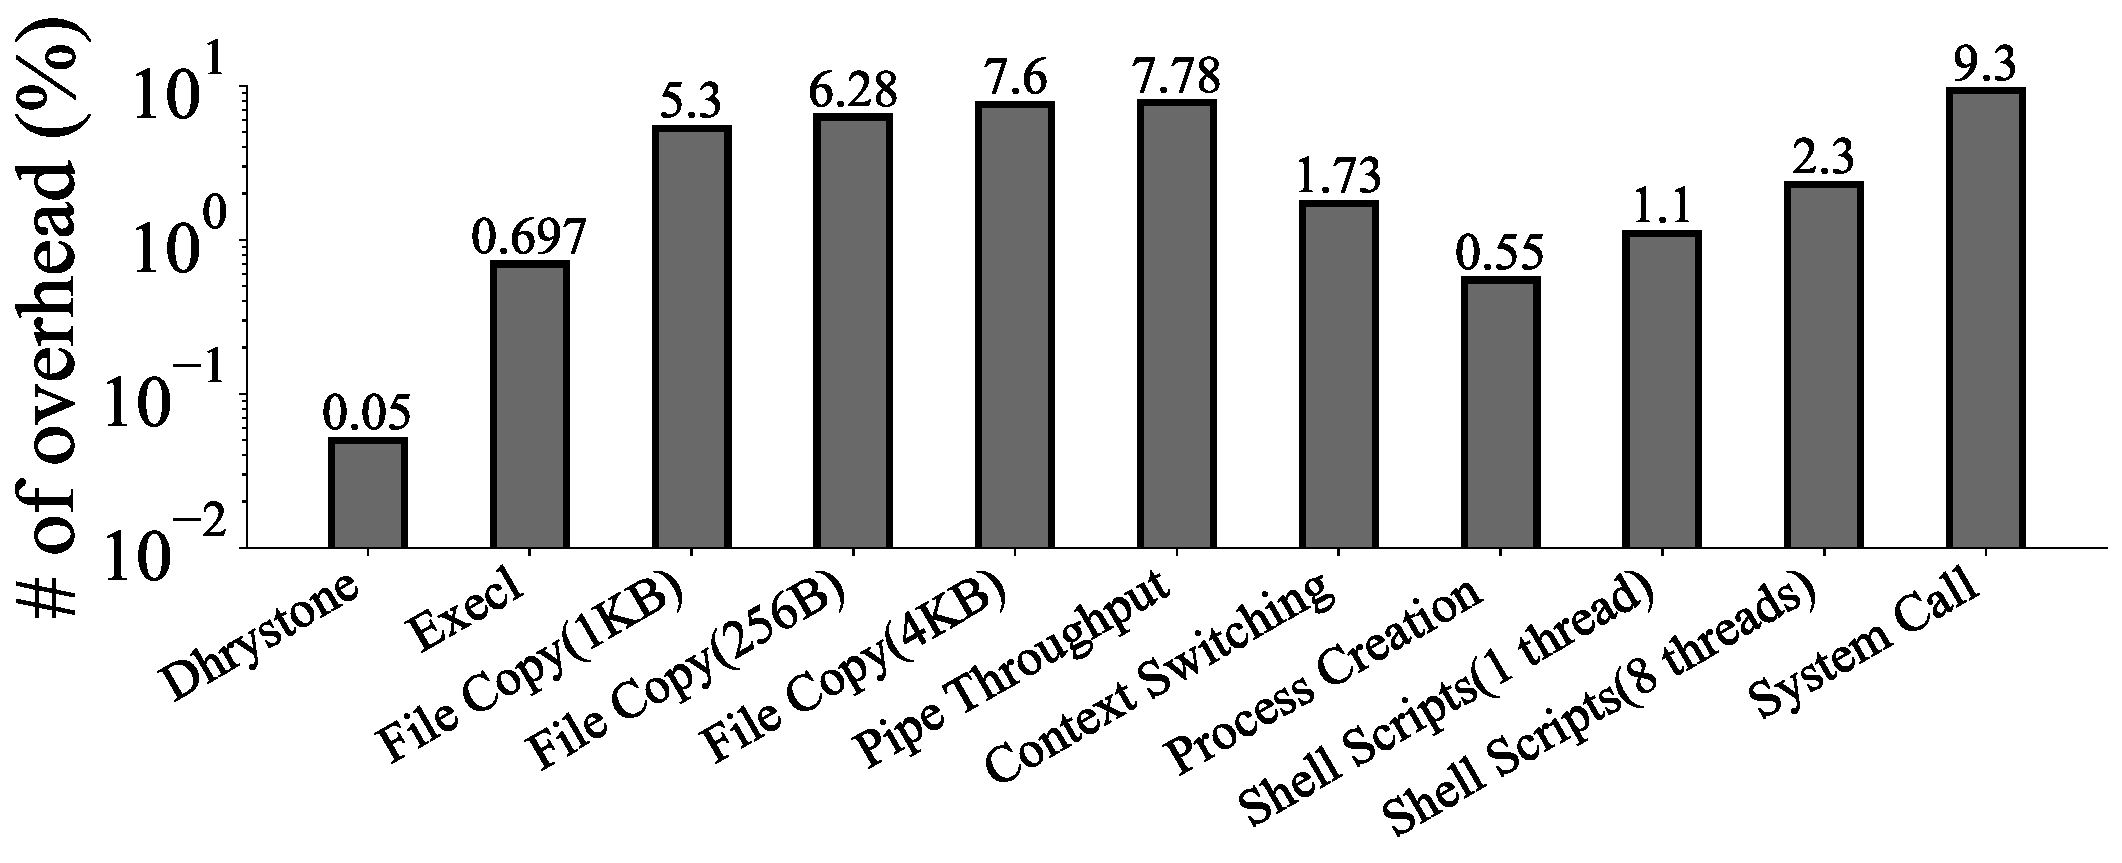
\includegraphics[width=0.9\textwidth]{figures/unixbenchoverheadbar.pdf}
    \caption{Performance overhead of running UnixBench with ETM tracing and non-deterministic event TheName.}
    \label{fig:Performance overhead of running UnixBench}
\end{figure}

We run UnixBench on Linux and show the performance results in Figure
\ref{fig:Performance overhead of running UnixBench}. For the tracing enabling,
the performance overhead is 3.88\% on average, and the highest performance
overhead is for System Call at 9.3\%. Specifically, there are three types of
benchmarks: File Copy, Pipe Throughput, and System Call that have higher
overhead. We believe that it is because these benchmarks have more frequent
\syscall{} invoking and I/O operations, which incur larger overhead than others.

\subsubsection{Nginx} \label{subsec:eva-Performance-Nginx}

We use \texttt{nginx} \cite{nginx_1.20.0} as a web server program to test the
performance of \TheName in a high concurrency environment. We use \texttt{ab}
(Apache HTTP server benchmarking tool) \cite{ApacheBench} to simulate user
access behavior. Setting \texttt{nginx} to its default configuration, we operate
performance testing with concurrency of 5,000 and request number of 500,000.

The average time cost for baseline (i.e., without \TheName) is 88.94s, and
\TheName is 90.09s with 1.30\% overhead. This shows that \TheName performs well
even in high-pressure environments.

\subsubsection{Performance overhead on real-world programs} \label{subsec:eva-Performance-Normal}

We use four real-world programs to test the \TheName for performance overhead of
normal executions, including \texttt{Pbzip2}, \texttt{Aget}, \texttt{SQLite},
and \texttt{Memcached}. We run different fine-grained tests on each of the
programs to simulate three different load scenarios. We run \texttt{Pbzip2} to
compress $10$MB, $500$MB, and $2$GB files, respectively. We use \texttt{Aget} to
download $50$MB, $500$MB, and $2$GB files in the same network to
avoid network speed interference. \texttt{SQLite} is evaluated by a
\texttt{sqlite-bench} \cite{sqlitebench} to write $100,000$, $500,000$, and
$2,000,000$ values in sequential key order in sync mode, respectively. A
benchmark tool \texttt{Twemperf} \cite{twemperf} was used to test
\texttt{Memcached}, which creates $20,000$, $300,000$, and $1,000,000$
connections to a Memcached server running on localhost.

\begin{figure}
    \centering
    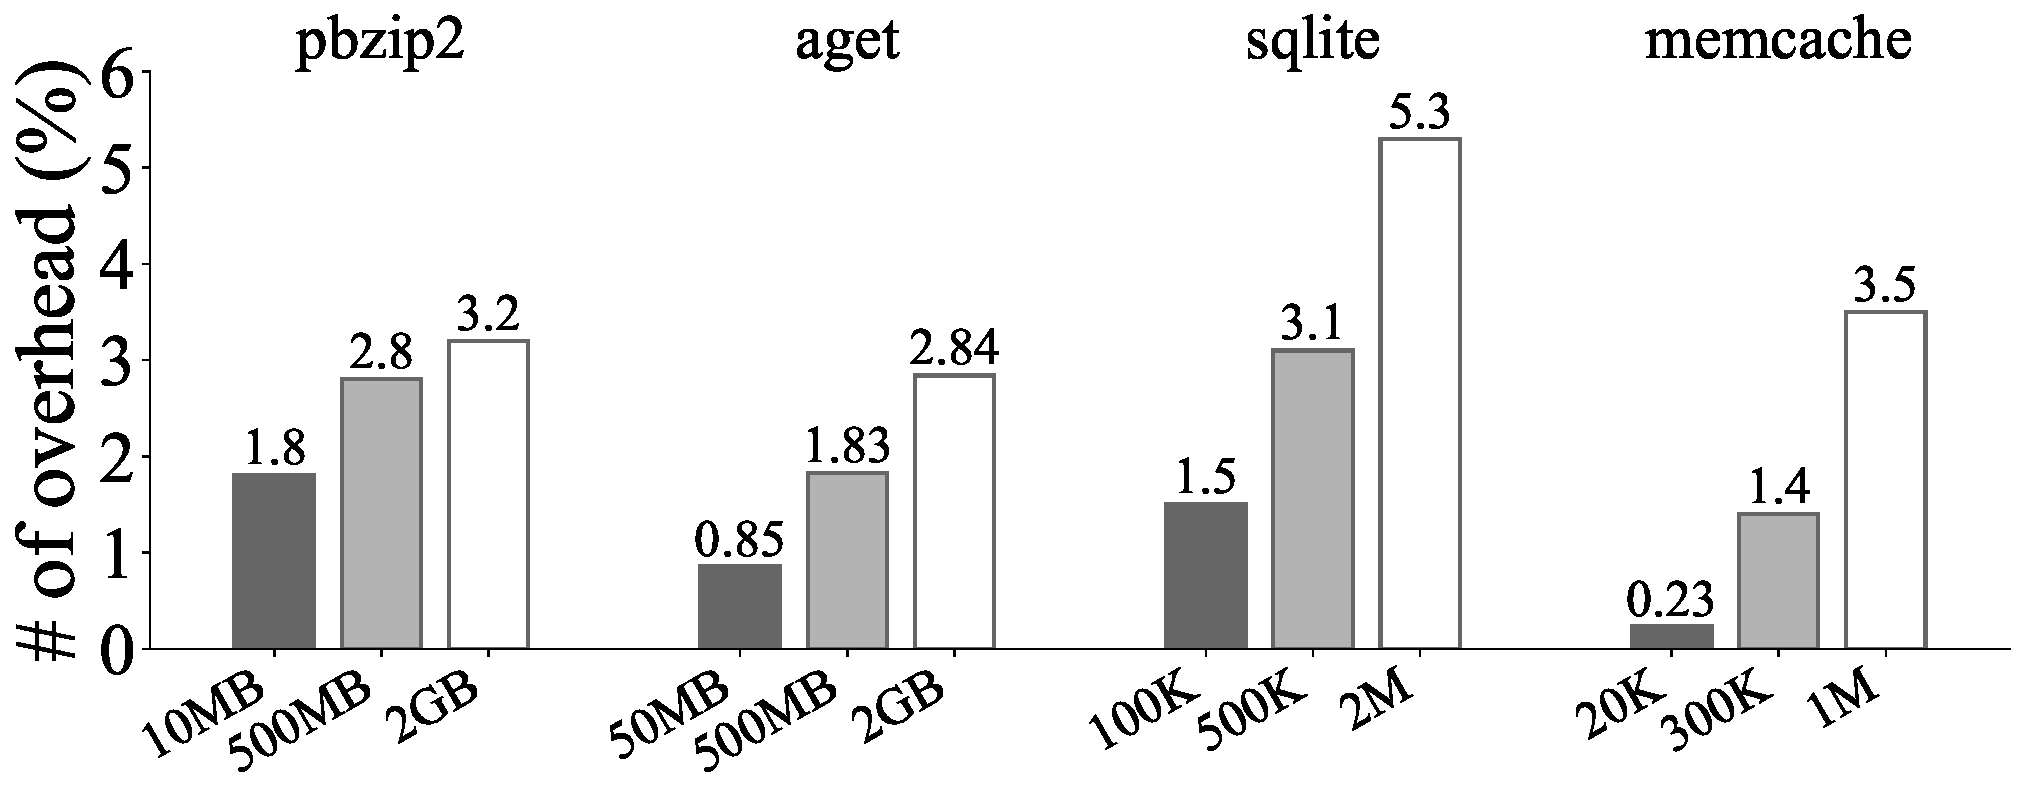
\includegraphics[width=0.9\textwidth]{figures/normaloverheadbar.pdf}
    \caption{Performance overhead of 4 real-world prgrams execution enables ETM tracing and non-deterministic event TheName with library hook.}
    \label{fig:Performance overhead of Normal Execution}
\end{figure}


We show performance overhead results in Figure \ref{fig:Performance overhead of
    Normal Execution}.
% For ETM tracing only, control flow tracing incurs a runtime
% performance overhead of 0.0071\% on average with no test exceeding 0.1\%
% overhead across all programs. 
Overall, the average performance overhead of all tests is 2.3\%, and the highest
overhead is 5.3\% for \texttt{SQLite} when writing $2,000,000$ values. The
performance overhead has a slight improvement when test stress increases in all
four programs. We believe it is caused by \TheName because there are many I/O
operations and a large number of \syscall{}s.
%cause more overhead
%than others.

%compare to REPT LAZY
We compare the runtime performance overhead of real-world programs with the
state-of-the-art systems \cite{cui2018rept, kasikci_lazy_2017}. The results show
that our overhead is slightly higher, mainly caused by the
\TheName. Nevertheless, \TheName still incurs a low runtime performance overhead
(2.3\% on average). We conclude this overhead is acceptable and still suitable for
practical deployment.

\subsubsection{Trade-offs Between Performance and Accuracy} \label{space-consumption}

% Since we collect a lot of data at runtime, we need to consider its consumption
% on space illustrate our trade-offs for \Recordingstage.

We design two versions of syscall capturing to record \textit{RC-Type}
\syscall{}s: saving the whole content or truncating to the beginning 256 bytes
. We test the time and space consumption of both
versions by a program that continuously reads a 2 GB text file to simulate a
highly concurrent environment on the server. The experimental results shown in
Table \ref{space_consumption} demonstrate that saving the entire content imposes
a significant overhead (12.5\%). In addition, an estimate for 24 hours of
continuous recording generates nearly 1 TB files, which indicates that saving
the entire content is also impractical for a larger throughput server.
Therefore, we choose to truncate the records of \textit{RC-Type} \syscall{}s to
the beginning 256 bytes.

\begin{table}[]
    % \small
    \caption{Space Consumption for Saving All Content or Truncation}
    \label{space_consumption}
    \centering
    \begin{tabular}{@{}llll@{}}
        \toprule
        \textbf{Type}        & \textbf{Real Time}       & \textbf{File Size} & \textbf{\begin{tabular}[c]{@{}l@{}}Estimated \\ 24-hour File Size\end{tabular}} \\ \midrule
        \textbf{Baseline}    & 2 min 50.3 s             & -                  & -                                  \\
        \textbf{All Content} & 3 min 11.552 s (+12.5\%) & 2.0 GB             & 902.1 GB                           \\
        \textbf{Truncation}  & 2 min 57.675 s (+4.33\%) & 120 MB             & 52 GB                              \\ \bottomrule
    \end{tabular}
\end{table}


\subsection{Generality} \label{subsec:eva-Generality}

% REPT,SNORLAX,POMP,WATCHER

% \begin{itemize}
%  \item Non-Intrusiveness (This makes SNORLAX non-invasive and therefore more practically applicable.)
%  \item semantic-aware handling of system calls
%  \item data flow recovery
%  \item Generality: Diagnose sequential or concurrency bug(MAV)
%  \item Reproduce Requiement (Watcher relies on a record-and-replay framework that can
% identically reproduce a failing execution.  If an application cannot be
% reproduced identically, then it is impossible to utilize Watcher to diagnosis
% failures of these applications.)
% \end{itemize}


\section{Discussion} \label{sec:discussion} 

This section discusses the limitations of \TheName and how I intend to address them in future work.

Currently, \TheName only considers 60 of 276 syscalls. Although I have already accounted for diverse types of system calls, handling more system calls is necessary to make \TheName becoming a practical system. Adding handlers for all system calls is the main task in the future.

Another limitation of \TheName is that it currently only supports system calls. Nevertheless, a similar approach with \TheName can handle other types of non-deterministic events. The
interrupts and traps can be dealt with by similar kernel hooks, and the signals
would require additional capturer in user-space. Moreover, the noninitialized variables are saved in memory, and therefore should appear in the coredump. Therefore, handling interrupts and traps is also one of my future work.

Currently, \TheName works perfectly on ARM devices. In my evaluation, it also runs normally on the x86 platform except for recording the return address. The only difference among these architectures is the approach to obtaining the registers differs. I will add supports for other platforms in the future.

Although \TheName performs well in common scenarios with only 5.3\% overhead at most, I can still apply many optimizations. For example, different record formats for different system calls are still a problem, and my current solution is to name each item. Therefore, records likes \texttt{pid=14311, accept4, res=3} (with the attribute name \texttt{pid} and \texttt{res}) additionally consumes a considerable amount of space. In the future, I need to classify the format of the record to reduce the space occupation of records.


In addition, \Filter of \TheName can only support limited conditions. To make \TheName more practical, some basic logic operators (e.g., \texttt{AND}, \texttt{OR} and \texttt{NOT}) should also be supported.

Finally, \TheName needs to have the ability to support long-term running. The size of the record file should not increase unlimitedly. Therefore, processing of historical recording data (dumping, compression, overwriting, etc.) will also be a future work.
\section{Related Work}

There is a large amount of related work to cpaturing syscalls. In this section, I discuss some representative examples and describe
how \TheName differs.

\textbf{Record and replay systems} are a type of systems that record sufficient information to reconstruct the program execution and then replay this execution. Record and replay systems are undoubtedly necessary to handle system calls or not replay faithfully.
Pinplay \cite{patil_pinplay_2010} is a record and replay system based on Pin  \cite{reddi_pin_2004}, a binary instrumentation system. While it does record system calls, the instrument-based approach introduces significant overhead (up to 140x). REPT \cite{cui_rept_2018} chooses to not record non-deterministic events such as system calls. In contrast, REPT adopts inference algorithms to reconstruct the effects of system calls. However, inference-based approaches can not achieve a 100\% reconstruction. For example, REPT can not deal with bugs like Figure \ref{fig:data-race}.

RR \cite{203227} is one of the-state-of-the-practice record and replay systems. RR perform the recording to non-deterministic events via \texttt{ptrace} \cite{ptrace2},
a \syscall{}
that allows a process to inspect and control the execution of another
one.
By using \texttt{ptrace}, a supervisory process can easily observe and intercept \syscall{}s issued by the target program.
Nevertheless,
% \zhenyu{what is "the supervisor"?}
\texttt{ptrace} brings a considerable overhead (up to 7.85×) as the supervisor also runs in
user space, 
% \zhenyu{why you write this? You introduced a tool, and then suddenly
% talk about some other things.}
which means that the supervisor needs to capture data with several
context switches (between target process with supervisor).

% \textbf{Linux troubleshooting tools} are a type of tools to inspect and record system status. Some Linux troubleshooting tools 
Some \textbf{Linux troubleshooting tools} monitor the target application and captures data
from non-deterministic events, such as Sysdig \cite{github_sysdig_2021}, DTrace
\cite{gregg_dtrace_2019,gregg_dtrace_2011}, and Strace \cite{github_strace_2021}.
Nevertheless, Strace \cite{github_strace_2021} also utilize \texttt{ptrace} to capture syscalls, which is similar to RR and inevitably introduces a considerable overhead. DTrace is powerful and efficient, but it is too sophisticated to use and require technical knowledge to optimize \cite{gregg_dtrace_2011}. Sysdig also leverages \textit{Linux tracepoints} as \TheName to achieve a relevant reasonable overhead (about 15\%); however, Sysdig sacrifices the completeness of its records, i.e., it does not guarantee that all system calls will always be recorded \cite{degioanni_sysdig_2014}.
% Nevertheless, these tools are desgined to
% monitor and troubleshoot applications, and performance is not their primary
% consideration.
% Nevertheless, some of these tools are designed to monitor and troubleshoot applications
% instead of precisely recording their effects \cite{github_sysdig_2021}; some do not concern about the runtime performance ; 
% others are hard to use and require technical knowledge to optimize \cite{gregg_dtrace_2011}.


% \begin{itemize}
%     \item \textbf{Pinplay} \dots
%     \item \textbf{REPT} \dots
%     \item \textbf{rr} \dots
%     \item \textbf{DTrace} \dots
%     \item \textbf{sysdig} \dots
% \end{itemize}


\section{Conclusion}

I propose a syscall record tool \TheName on ARM to satisfy practical requirements. It takes advantage of the mechanisms in Linux to completely and efficiently capture and record system calls. \TheName achieves its design goals and is suitable as the basis for record and replay systems. 
\clearpage
\参考文献
% \nocite{*}
  \printbibliography[heading=none]
  \clearpage
\附录
  % !Mode:: "TeX:UTF-8"
% !TEX program  = xelatex

% \section*{数据获取函数}\label{A:data}
% \Python{utils.py}{code/examples/utils.py}
\section*{Source Code}
\TheName is an open source proejct on Github: its source code can be found at https://github.com/Tert-butyllithium/syscord\clearpage
\致谢
  \TheName is an important part of another project, which is submitted to ACM CCS 2021. Thanks to my collaborators, including Yiming Zhang, Wenxuan Shi, Yuxin Hu, and Xueying Zhang. I have learned a lot from the project. Besides, Yiming as the first user of \TheName has also raised many issues for \TheName, which makes \TheName better.

I would like to express my gratefulness to my advisor, Dr. Fengwei Zhang, for his continuous support and encouragement during my college life in SUSTech.  Dr. Zhang's encouragement has rekindled my passion for research and eventually motivated me to continue on my research path. Dr. Zhang provided a lot of time to discuss with me when I was facing difficulties in research and life.

I am very appreciative to Dr. Zhenyu Ning for his guidance in our project. Dr. Ning's insightful and critical suggestions are an essential factor in making this project successful. Dr. Ning's enthusiasm, modest and gentle, has also influenced me in my life and research.

Moreover, I would like to thank all the group members in COMPASS Lab. I have joined COMPASS Lab a year ago and it has been a pleasant and impressive experience with every genius in the lab. 

Meanwhile, I treasure my nearly two years of training at SUSTech-CPC, and I would like to thank every member of the training team and my coach, Dr. Bo Tang. Although I didn't achieve the expected results, the continuous practice has improved my comprehensive programming proficiency. More importantly, I have encountered many good friends in the team, who gave me a lot of support and encouragement and helped me get through the most miserable period.



Also, I deeply appreciate to my girl friend, who has been absent for 21 years of my life. Therefore I can only focus on my work. 
\end{document}
